%
 
Niniejszy rozdział poświęcony jest opisowi aplikacji powstałej na podstawie wymagań sformułowanych w opisie pomiaru (link). Analiza wymagań podyktowała stworzenie programu, który umożliwiałby pogląd ramek zarządzających komunikacją w standardzie 802.11 (ang. \emph{Management frames}) oraz analizę zależności czasowych między nimi. 

Wymagane okazało się stworzenie aplikacji nasłuchującej (ang. \emph{sniffer}) przystosowanej do obserwacji typowych scenariuszy zachodzących w komunikacji w medium bezprzewodowym. Przystosowanie to rozumiem jako możliwość konfiguracji programu pod kątem wybranego zjawiska i środowiska pomiarowego. 

\subsection{Środowisko pracy programu.}

Program hop-sniffer został przygotowany dla systemu operacyjnego Linux w wersji jądra 2.6. W wyborze systemu operacyjnego kierowałem się głównie metodą implementacji sterowników urządzeń bezprzewodowych i obsługującej je warstwy pośredniej jądra. 

System Linux był wyborem oczywistym ze względu na możliwość konfiguracji interfejsów NIC w sposób umożliwiający przetwarzanie ramek typu MGMT (ang. \emph{management}) standardu 802.11 za pomocą aplikacji w przestrzeni użytkownika.

Kolejną zaletą wybranego systemu jest możliwość konfiguracji najbardziej odpowiedniej dystrybucji i kompilacji powstałego rozwiązania jedynie z użyciem opcji dedykowanych dla aplikacji pomiarowej. W tym wypadku najbardziej pożądane jest minimalistyczne środowisko, które w możliwie najmniejszym stopniu wpływało będzie na prezentowane przez program wyniki pomiarów. Jako środowisko zalecane wybrałem system Arch Linux (link).

Biorąc pod uwagę program komunikujący się z kartą radiową w systemie Linux należy zwrócić szczególną uwagę na kwestię sterowników. Od sterowników urządzeń bezprzewodowych zależy jakie polecenia i tryby pracy interfejsów będą dostępne do konfiguracji w przestrzeni użytkownika. Ze względu na aktualne dążenie programistów jądra do unifikacji interfejsu obsługi urządzeń standardu 802.11 powstała warstwa pośrednia \emph{mac80211}. Postanowiłem oprzeć aplikację hop-sniffer o sterowniki działające w tej warstwie ze względu na wspólny, oparty na gniazdach interfejs komunikacyjny \emph{nl80211}. Kluczowym wymaganiem stawianym sterownikowi jest implementacja polecenia umożliwiającego utworzenie wirtualnego interfejsu karty radiowej pracującego w trybie \emph{monitor}.

Wprowadzenie karty radiowej w tryb \emph{promiscuous} powoduje jedynie wyłączenie filtracji adresów MAC. Program hop-sniffer musi mieć możliwość odbierania ramek standardu 802.11 bez potrzeby asocjacji z SSID (ang. \emph{Service Set Identifier}) żadnej sieci. Wyłączenie filtracji SSID możliwe jest jedynie w trybie \emph{monitor}.

W swojej pracy skoncentrowałem się na współpracy ze sterownikiem \emph{ath9k}. Jest to całkowicie otwarty sterownik do urządzeń standardu 802.11bgn firmy \emph{Atheros}. Za wykorzystaniem sterownika przemawia dostępność wspieranych przez niego urządzeń, implementacja szerokiej gamy poleceń interfejsu \emph{nl80211} oraz możliwość pracy w trybie \emph{monitor}.

\subsection{Biblioteki programistyczne.}

Implementacja aplikacji pomiarowej wymagała zastosowania API (ang. \emph{Application interface}) umożliwiającego pochwycenie ramek zarządzających komunikacją 802.11 w przestrzeni użytkownika. Podczas procesu tworzenia programu hop-sniffer rozpatrzyłem zastosowanie dwóch bibliotek: \emph{libnl} i \emph{libpcap}.

\subsubsection{Nasłuchiwanie za pomocą interfejsu \emph{nl80211}.}

\emph{Libnl} jest to API (ang. \emph{Application interface}) służące do komunikacji między przestrzenią użytkownika i warstwą \emph{mac80211} jądra systemu operacyjnego. Interfejs \emph{nl80211} tej warstwy oparty jest o system gniazd \emph{Generic Netlink} (w odróżnieniu od stosowanych dawniej wywołań systemowych \emph{IOCTL}).  

Warstwa pośrednia definiuje rodzinę gniazd (ang. \emph{Generic netlink family}) oraz rejestruje w jej obrębie zestaw poleceń w postaci akceptowanych rodzajów wiadomości. Sterowniki urządzeń 802.11 implementują powyższy interfejs poprzez inicjalizację odpowiadających poleceniom wskaźników na funkcje własnymi operacjami. Każda wiadomość akceptowana przez daną rodzinę posiada własną nazwę oraz wskaźnik na strukturę określającą ilość i typy atrybutów (ang. \emph{Generic netlink attribute policy}), która pełni funkcję kontroli poprawności. Struktura ta zwana \emph{nla\_policy} stanowi wytyczne co do sposobu konstrukcji skierowanego do jądra polecenia oraz ekstrakcji danych z odebranej wiadomości.

W wyniku analizy dokumentacji uznałem, że możliwa będzie implementacja programu nasłuchującego z wykorzystaniem następujących mechanizmów udostępnianych przez interfejs \emph{nl80211}:

\begin{itemize}
\item[--] Grupowych adresów (ang. \emph{Multicast groups}) odbiorców wiadomości.
\item[--] Komendy \emph{NL80211\_CMD\_REGISTER\_FRAME}.
\item[--] Własnych funkcji obsługi zdarzeń (ang. \emph{Custom callback}).
\item[--] Komendy \emph{NL80211\_CMD\_FRAME}.
\end{itemize}

Adresy grupowe są wykorzystywane przez jądro do rozgłaszania zdarzeń warstwy \emph{mac80211} do zainteresowanych procesów (posiadających gniazdo z członkostwem w danej grupie rozgłaszania). W celu otrzymywania wszystkich zdarzeń należy zarejestrować gniazdo (\ref{code:MulticastExample}) we wszystkich czterech grupach: \emph{Configuration, Scan, Regulatory i MLME}. Podczas rejestracji (\ref{code:MulticastExample}) funkcja \emph{nl\_get\_multicast\_id(3)} przyjmuje uchwyt gniazda komunikacyjnego, nazwę rodziny, do której odnosi się zapytanie i nazwę grupy, której identyfikator chcę uzyskać. W wyniku wywołania otrzymuję liczbę całkowitą, którą mogę wykorzystać w celu rejestracji danego gniazda w grupie rozgłaszania przy pomocy funkcji \emph{nl\_socket\_add\_membership(2)}.

\lstset{caption={Przykład rejestracji gniazda w grupie \emph{Configuration}.}, label={code:MulticastExample}}
\begin{lstlisting}[frame=tb]
/* Get configuration multicast group ID */
multicast_id = nl_get_multicast_id(cd->nl_sock, 
        "nl80211", "config");
if (multicast_id < 0)
        return multicast_id;
                                        
/* Add membership to configuration multicast group */
ret = nl_socket_add_membership(cd->nl_sock, multicast_id);
if (ret)
        return ret;
\end{lstlisting}

Komenda \emph{NL80211\_CMD\_REGISTER\_FRAME} pozwala na rejestrację wybranych typów ramek do przetwarzania w przestrzeni użytkownika. Wymagane atrybuty to indeks interfejsu radiowego (\emph{NL80211\_ATTR\_IFINDEX} to liczba całkowita 32-bitowa), typ ramki (\emph{NL80211\_ATTR\_FRAME\_TYPE} to liczba całkowita 16-bitowa) oraz wzorca zawierającego pierwsze bajty ramki (\emph{NL80211\_ATTR\_FRAME\_MATCH} to wzorzec binarny z podaną długością), które powinny być dopasowane. Należy wziąć pod uwagę fakt, że w tym wypadku aplikacja musi obsłużyć dany typ ramek, gdyż nie zostaną one odpowiednio przetworzone w jądrze. Zamknięcie gniazda komunikacyjnego za pomocą, którego dokonano rejestracji powoduje jej porzucenie. 

W mojej aplikacji zgłaszanie ramek do obsługi przez program nasłuchujący jest częścią inicjalizacji. Należy zarejestrować wszelkie ramki niezbędne do obserwacji wybranego zjawiska. Proces budowania wiadomości (\ref{code:RegisterFrame}) zaczyna się od stworzenia nagłówka opatrzonego odpowiednim adresem odbiorcy (identyfikatorem rodziny) oraz nazwą polecenia do wykonania. Służy do tego funkcja biblioteczna \emph{genlmsg\_put(8)}, która dodaje do otrzymanego uchwytu wiadomości nagłówek wybranej komendy przynależącej do identyfikatora podanej rodziny. Następnie dodaję atrybuty wymagane przez komendę specyfikując identyfikator (potrzebny w celu sprawdzenia poprawności) oraz wartość. Są one wstawiane do pól wiadomości za pomocą makr bibliotecznych \emph{NLA\_PUT} (odpowiadających typowi danych). Numer interfejsu tłumaczony jest z nazwy (np. \emph{wlan0}) na indeks (typ całkowity). Rodzaj ramki to liczba całkowita 16-bitowa, którą w języku C możemy wprowadzić \emph{in-situ} jako \emph{0x0040} (ramka typu \emph{Probe Request}). Po zbudowaniu prawidłowej wiadomości pozostaje wysłać ją za pomocą funkcji bibliotecznej \emph{nl\_send\_auto\_complete(2)}. 

\lstset{caption={Przykład rejestracji ramki do obsługi w przestrzeni użytkownika.}, label={code:RegisterFrame}}
\begin{lstlisting}[frame=tb]
/* Build netlink message header */
genlmsg_put(msg, 0, 0, genl_family_get_id(cd->nl80211), 
        0, 0, NL80211_CMD_REGISTER_FRAME, 0);
/* Device interface index to use */
devid = if_nametoindex(if_name);
NLA_PUT_U32(msg, NL80211_ATTR_IFINDEX, devid);
/* Register frame type/subtype */
NLA_PUT_U16(msg, NL80211_ATTR_FRAME_TYPE, fr_type);
/* Frame match for MGMT frames is NULL */
NLA_PUT(msg, NL80211_ATTR_FRAME_MATCH, 0, NULL);       
/* Send message */
error = nl_send_auto_complete(cd->nl_sock, msg);
\end{lstlisting}

Po przyłączeniu gniazda do odpowiednich grup rozgłaszania i wybraniu niezbędnych typów ramek do przetwarzania przez program pozostaje rozpocząć nasłuchiwanie zdarzeń interfejsu \emph{nl80211} (\ref{code:ListenEvents}). W mojej aplikacji wybór badanego zjawiska (sposobu reakcji na zdarzenia) zależy od rodzaju funkcji do której wskaźnik jest przekazywany podczas rozpoczęcia nasłuchu. Funkcja ta przekazywana jest jako argument procedury typu \emph{callback} używanej do przetwarzania odebranych wiadomości (zdarzeń). 

Zdefiniowana przeze mnie funkcja \emph{custom\_event\_handler} zostaje wybrana do obsługi zdarzeń za pomocą procedury bibliotecznej \emph{nl\_cb\_set(5)} z flagami \emph{NL\_CB\_VALID} (używana do wiadomości poprawnych) i \emph{NL\_CB\_CUSTOM} (zdefiniowana przez użytkownika). Dodatkowo przekazuję wskaźnik na stworzone przez siebie argumenty wywołania (w tym uchwyt do funkcji obsługującej obserwację wybranego zjawiska \emph{fptr\_handle\_frame}), które będą dostępne w bloku procedury \emph{custom\_event\_handler}. Blokująca procedura biblioteczna \emph{nl\_recvmsgs} oczekuje na zdarzenia i wywołuje dla nich przekazaną jej funkcję \emph{callback}. 

\lstset{caption={Fragment kodu procedury rozpoczynającej obsługę zdarzeń.}, label={code:ListenEvents}}
\begin{lstlisting}[frame=tb]
/* Choose scenario type. */
args.handle_frame = fptr_handle_frame;
/* ... */
/* set custom event handler and pass arguments to it. */
nl_cb_set(cb, NL_CB_VALID, NL_CB_CUSTOM,
        custom_event_handler, &args);
/* ... */
/* Listen events. */
while (!command)
{
        nl_recvmsgs(cd->nl_sock, cb);
}
\end{lstlisting}

Komenda \emph{NL80211\_CMD\_FRAME} służy do nadawania i odbierania wybranych typów ramek z poziomu aplikacji użytkownika. W przypadku programu nasłuchującego interesuje mnie funkcjonowanie tej wiadomości jako zdarzenia propagowanego przez jądro w sytuacji otrzymania nieobsłużonej ramki. 

Odebranie przez nasłuchujące gniazdo poprawnej wiadomości interfejsu \emph{nl80211} powoduje wywołanie własnej funkcji obsługi \emph{custom\_event\_handler} (\ref{code:EventHandler}). Celem jest rozpoznanie komendy \emph{NL80211\_CMD\_FRAME} i przekazanie jej atrybutu \emph{NL80211\_ATTR\_FRAME} do funkcji obsługujące obserwowane zjawisko. Atrybut \emph{NL80211\_ATTR\_FRAME} reprezentuje odebraną ramkę (nagłówek i pole danych) i jest typu binarnego (ciąg bajtów). 

Pierwszym krokiem jest ekstrakcja nagłówka wiadomości \emph{netlink} w postaci argumentu wywołania i jego rozpakowanie  do postaci struktury \emph{genlmsghdr} za pomocą funkcji bibliotecznych \emph{nlmsg\_hdr(1)} i \emph{nlmsg\_data(1)}. Struktura ta zawiera pole \emph{cmd} będące identyfikatorem komendy, którego używam w bloku \emph{switch}.

Niezbędna jest ekstrakcja atrybutów wiadomości za pomocą procedury bibliotecznej \emph{nla\_parse(5)}, która otrzymuje bufor na atrybuty (mogący pomieścić \emph{NL80211\_ATTR\_MAX} + 1 atrybutów), stałą biblioteczną oznaczającą liczbę wszystkich atrybutów \emph{NL80211\_ATTR\_MAX}, początek listy atrybutów (struktura \emph{nlattr}) znaleziony za pomocą funkcji bibliotecznej \emph{genlmsg\_attrdata(2)} i długość listy atrybutów otrzymana z wykorzystaniem funkcji \emph{genlmsg\_attrlen(2)}. Otrzymaną w ten sposób tablicę struktur \emph{nlattr} indeksuję identyfikatorem atrybutu \emph{NL80211\_ATTR\_FRAME} przekazuję go jako argument wywołania funkcji obsługującej obserwowane zjawisko \emph{handle\_frame} przekazanej w zdefiniowanej wcześniej strukturze argumentów użytkownika \emph{event\_handler\_args}. 

\lstset{caption={Własna funkcja obsługi zdarzeń.}, label={code:EventHandler}}
\begin{lstlisting}[frame=tb]
int custom_event_handler(struct nl_msg *msg, void *arg)
{
    /* Generic netlink message header */
    struct genlmsghdr *gnlh = nlmsg_data(nlmsg_hdr(msg));
    /* Buffer for attributes from netlink message */
    struct nlattr *msg_attr_buff[NL80211_ATTR_MAX + 1];
    struct event_handler_args *args = arg;
        
    /* Extract attributes */
    nla_parse(msg_attr_buff, 
              NL80211_ATTR_MAX, 
              genlmsg_attrdata(gnlh, 0), 
              genlmsg_attrlen(gnlh, 0), 
              NULL);
        
    /* Handle event according to type */
    switch (gnlh->cmd) 
    {
    /* ... */
    case NL80211_CMD_FRAME:
        if(msg_attr_buff[NL80211_ATTR_FRAME])
            args->handle_frame(
                msg_attr_buff[NL80211_ATTR_FRAME]);
        break;
    /* ... */
    }
/* ... */
}
\end{lstlisting}

Przykładowym sposobem obsługi wybranego zjawiska komunikacji bezprzewodowej w standardzie 802.11 jest procedura \emph{handle\_frame} (\ref{code:HandleFrame}). Przekazanie funkcji obsługi poprzez wskaźnik jest sposobem na różnicowanie działania programu w zależności od scenariuszy komunikacyjnych, które są obiektem badań oraz dostarczenie ujednoliconego interfejsu ich implementacji. 

Głównym krokiem procedury jest ekstrakcja atrybutu \emph{nl80211} reprezentującego ramkę standardu 802.11 do postaci ciągu bajtów za pomocą funkcji bibliotecznej \emph{nla\_data(1)}. Otrzymana w ten sposób tablica jest indeksowana w poszukiwaniu konkretnych bajtów, a ekstrakcja informacji polega na zastosowaniu maski bitowej (przykładowo \emph{0xfc} do bajtu podtypu). 

\lstset{caption={Funkcja \emph{handle\_frame}.}, label={code:HandleFrame}}
\begin{lstlisting}[frame=tb]
void handle_frame(struct nlattr *nl_frame)
{
	uint8_t *frame;
        /* ... */
        /* Extract frame byte array from netlink attribute */
	frame = nla_data(nl_frame);
        /* ... */
	switch (frame[0] & 0xfc) 
        {
	        case 0x10: /* assoc resp */
                        /* ... */
                        break;
                case 0xa0: /* disassoc */
                        /* ... */
                        break;
        }
}
\end{lstlisting}

Stworzona przeze mnie aplikacja oparta na powyżej opisanej metodyce spełniała założenia powstałe w fazie analizy wymagań dla testowanych ramek standardu 802.11 typu \emph{Probe Request}. Niestety rejestracja ramek dla interfejsu typu \emph{monitor} okazała się niemożliwa, a typy ramek możliwe do odbierania na poszczególnych interfejsach (ang. \emph{Supported RX frame types}) są całkowicie zależne od implementacji sterownika i mocno ograniczone ze względu na jego typ. Aktualnie typy ramek 802.11 możliwe do wysyłania i dobierania na danym interfejsie są dostępne i ogłaszane w atrybutach wirtualnego urządzenia reprezentującego kartę radiową (ang. \emph{Wiphy}). Urządzenie to jest zaimplementowane w warstwie pośredniej \emph{mac80211}, a struktury je opisujące wypełniane są przez odpowiadający mu sterownik.

% MARGINES
Inspekcja dostępnych w przestrzeni użytkownika ramek możliwa jest dzięki analizie odpowiedzi interfejsu \emph{nl80211} na komendę \emph{NL80211\_CMD\_GET\_WIPHY} z dodatkową flagą nagłówka \emph{netlink} o nazwie \emph{NLM\_F\_DUMP}, która powoduje przekazanie do wysyłającej aplikacji wiadomości ze wszystkimi parametrami wybranych urządzeń \emph{Wiphy}.

\lstset{caption={Część atrybutów \emph{Wiphy} o identyfikatorze \emph{phy0} (program \emph{iw-3.2}).}, label={code:WiphyAttributes}}
\begin{lstlisting}[frame=tb]
marcin@marcin-PC:~/iw-3.2$ ./iw phy0 info
Wiphy phy0
        ...
	Supported RX frame types:
		 * IBSS: 0x00d0
		 * managed: 0x0040 0x00d0
		 * AP: 0x0000 0x0020 0x0040 0x00a0 0x00b0 
                   0x00c0 0x00d0
		 * AP/VLAN: 0x0000 0x0020 0x0040 0x00a0 
                   0x00b0 0x00c0 0x00d0
		 * mesh point: 0x00b0 0x00c0 0x00d0
		 * P2P-client: 0x0040 0x00d0
		 * P2P-GO: 0x0000 0x0020 0x0040 0x00a0 
                   0x00b0 0x00c0 0x00d0
	...
\end{lstlisting}

Analiza dostępnych do odebrania ramek wskazuje, że nie jest możliwe badanie niektórych zjawisk (np. roaming 802.11). Interfejsy nie pozwalają na rejestrację w jądrze ramek typu \emph{Association Response} (identyfikator \emph{0x1}), a odbieranie ramek typu \emph{Disassociation} (identyfikator 0xA) wymaga wprowadzenia interfejsu w tryb \emph{Master} (uruchomienia programu \emph{hostapd}, a więc utworzenia na komputerze punktu dostępowego). 

Oczywiście, jeśli nasłuchiwanie nie będzie prowadzone w trybie \emph{monitor} to program i tak nie otrzyma ramek z sieci, której nie jest członkiem (ze względu na filtrację SSID). 

Powyższe problemy powodują, że mimo uniwersalności i licznych zalet związanych z prostym sposobem ekstrakcji danych z ramek standardu 802.11 biblioteka \emph{libnl} nie nadaje się do zastosowania w aplikacji opisanej wymaganiami sformułowanymi w fazie opisu procedury pomiarowej (link). 

\subsubsection{Nasłuchiwanie za pomocą biblioteki typu \emph{pcap}.}

Biblioteka \emph{libpcap} (ang. \emph{Packet capture library}) udostępnia wysokopoziomowy interfejs przechwytywania pakietów (również tych, które nie są kierowane do danej maszyny) co czyni ją odpowiednim narzędziem do implementacji programu hop-sniffer. 

Procedura inicjalizacji programu nasłuchującego wymaga podjęcia następujących kroków:
\begin{enumerate}
\item Przygotowanie wirtualnego interfejsu pomiarowego w trybie \emph{monitor}.
\item Utworzenia urządzenia przechwytującego.
\item Ustalenie długości migawki.
\item Wprowadzenie interfejsu radiowego w tryb \emph{promiscuous}.
\item Ustalenie niedoczasu dla urządzenia przechwytującego.
\item Aktywacja urządzenia przechwytującego.
\item Sprawdzenie długości migawki.
\item Sprawdzenie przynależności do sieci.
\item Kompilacja kodu filtra pakietów.
\item Ustalenie skompilowanego filtra w urządzeniu przechwytującym.
\item Uruchomienie pętli głównej programu.
\end{enumerate}

Przygotowanie interfejsu pomiarowego może być wykonane poza programem za pomocą narzędzia konfiguracji interfejsów \emph{iw} (link). Interfejs w trybie \emph{monitor} tworzy się (\ref{code:MakeMonitor}) poprzez podanie nazwy istniejącego interfejsu radiowego, dzięki czemu możliwa jest identyfikacja urządzenia \emph{Wiphy}, które ma być współdzielone. 

\lstset{caption={Dodanie interfejsu \emph{mon0} w trybie \emph{monitor}}, label={code:MakeMonitor}}
\begin{lstlisting}[frame=tb]
marcin@marcin-PC:~$ iw dev wlan0 interface add mon0 type monitor
\end{lstlisting}

Podstawowym krokiem programu jest utworzenie uchwytu do urządzenia przechwytującego. Zadanie to polega na inicjalizacji wskaźnika na strukturę \emph{pcap\_t}. Struktura ta zdefiniowana jest w bibliotece w sposób nietransparentny (ang. \emph{opaque structure}), więc jej zawartość deklarowana jest w plikach źródłowych, a nie nagłówkowych. Funkcja tworząca urządzenie (\ref{code:PcapCreate}) przyjmuje tablicę znaków określającą nazwę interfejsu oraz tablicę bajtów przeznaczoną na kody ewentualnych błędów. 

\lstset{caption={Utworzenie uchwytu urządzenia przechwytującego}, label={code:PcapCreate}}
\begin{lstlisting}[frame=tb]
/* Create capture device */
pdev = pcap_create(device, ebuf);
\end{lstlisting}

Pierwszą z ważnych do ustalenia opcji jest długość migawki (ang \emph{snapshot length}). Długość wystarczająca do przechwycenia całej ramki wynosi \emph{65000} (\ref{code:PcapInit}). Zdecydowałem się na przechwytywanie całych ramek ze względu na przyszły rozwój aplikacji. Aktualnie nie jest możliwe do ustalenia do jakich typów pakietów będzie używany program. Rozmiar ramek zmienia się w zależności od użytych metod szyfrowania oraz zawartości nagłówka \emph{radiotap}. Użyta funkcja biblioteczna \emph{pcap\_set\_snaplen(2)} przyjmuje uchwyt do urządzenia oraz zmienną typu \emph{long long} reprezentującą długość migawki. 

% Czemu 65000 ? Czego ? Jak się zmienia rozmiar ? (przykłady).

Następnie należy wprowadzić urządzenie w tryb \emph{promiscuous} i ustalić niedoczas dla przechwytywania. Niedoczas określa odstępy w jakich biblioteka będzie dokonywała odczytów z urządzenia nasłuchującego. Nie jest to parametr, który zakłóca pomiar, gdyż czas otrzymania ramki odczytywany jest ze znacznika w nagłówku \emph{pcap}, a nie naliczany w aplikacji pomiarowej. Wartość 1000 milisekund pozwala na równomierne czytanie z bufora pakietów. Ustawień dokonuje się w sposób analogiczny podając uchwyt urządzenia przy wywołaniu funkcji \emph{pcap\_set\_promisc(2)} z wartością 1 (aby ustawić tryb \emph{promiscuous}) lub \emph{pcap\_set\_timeout(2)} z wartością 1000 (aby ustawić niedoczas 1000 milisekund).

\lstset{caption={Inicjalizacja parametrów urządzenia przechwytującego.}, label={code:PcapInit}}
\begin{lstlisting}[frame=tb]
/* Init capture device */
/* Set snapshot length */
err = pcap_set_snaplen(pdev, snapshot_size);
/* ... */
/* Set promiscus mode */
err = pcap_set_promisc(pdev, 1);
/* ... */
/* Set timeout */
err = pcap_set_timeout(pdev, 1000);
\end{lstlisting}

Na zakończenie procesu inicjalizacji uchwytu urządzenia należy go aktywować (\ref{code:PcapActivate}). Jest to okazja do obsługi wszelkich ostrzeżeń i błędów wygenerowanych w wyniku ustawionych powyżej opcji. Pomyślna aktywacja pozwala na rozpoczęcie nasłuchu w medium pracy wybranego interfejsu. Do błędów zaliczam wszelkie sytuacje, które nie pozwolą na dalszą poprawną pracę programu, a więc następujące wartości zwracane:
\begin{itemize}
\item[--] {\bf PCAP\_ERROR\_NO\_SUCH\_DEVICE:} Podana nazwa interfejsu nie istnieje. 
\item[--] {\bf PCAP\_ERROR\_PERM\_DENIED:} Użytkownik wywołujący program nie posiada uprawnień do otwarcia wybranego interfejsu.
\item[--] {\bf PCAP\_ERROR:} Błąd, który nie jest zdefiniowany w nagłówku biblioteki. 
\end{itemize}
Ostrzeżenia pozwalają na dalszą pracę programu, ale mogą poważnie ograniczyć jego funkcjonalność:
\begin{itemize}
\item[--] {\bf PCAP\_WARNING\_PROMISC\_NOTSUP:} Tryb interfejsu \emph{promiscuous} nie jest wspierany przez dostępne urządzenie. Będzie miała miejsce filtracja adresów MAC.
\item[--] {\bf PCAP\_WARNING:} Ostrzeżenie, które nie jest zdefiniowane w nagłówku biblioteki.
\end{itemize}

\lstset{caption={Aktywacja urządzenia przechwytującego.}, label={code:PcapActivate}}
\begin{lstlisting}[frame=tb]
/* Activate capture device */                                        
err = pcap_activate(pdev);
\end{lstlisting}

Po uruchomieniu urządzenia nasłuchującego należy sprawdzić część parametrów związanych z aktywacją (\ref{code:PcapCheck}). Po pierwsze rozmiar migawki, ponieważ mógł on ulec zmianie. Następnie fakt przynależności wybranego interfejsu przechwytywania do sieci. Rozmiar migawki pobiera się wykorzystując funkcję \emph{pcap\_snapshot(1)} podając uchwyt urządzenia. Podglądu sieci dokonuję wywołując procedurę \emph{pcap\_lookupnet(4)} z argumentem nazwy interfejsu, wskazania na 32-bitowe liczby całkowite reprezentujące sieć i jej maskę (do wypełnienia przez wywołanie) oraz tablicę bajtów na kod ewentualnych błędów. Kroki te są wykonywane w celach prezentacji informacji i mogą wygenerować jedynie ostrzeżenia.

\lstset{caption={Sprawdzenie parametrów po aktywacji urządzenia.}, label={code:PcapCheck}}
\begin{lstlisting}[frame=tb]
/* Check snapshot size after init */
i = pcap_snapshot(pdev);
/* ... */
/* Check sniffed network */
if (pcap_lookupnet(device, &localnet, &netmask, ebuf) < 0) 
{
/* ... */
}
\end{lstlisting}

Biblioteka \emph{libpcap} udostępnia kompilator reguł logicznych opisu filtrów na język BPF (ang. \emph{Berkley packet filter}). Jest on interesujący z perspektywy mojego programu ze względu na potrzebę maksymalnej redukcji opóźnień. Wprowadzenie instrukcji warunkowych do kodu programu w celu filtracji pakietów gdy jądro i tak przekazuje wszystkie przechwycone pakiety jest bardzo nieefektywne. 

Jądro systemów operacyjnych z pod znaku BSD (ang. \emph{Berkley Software Distribution} posiada wbudowany mechanizm szybkiej filtracji dostępny w postaci urządzeń \emph{/dev/bpf0}, \emph{/dev/bpf1} itd.  Zezwalają one na powiązanie zdefiniowanego przez użytkownika filtra pakietów. Asocjacja deskryptora urządzenia \emph{bpf} z otwartym gniazdem powoduje wpływ jego reguł filtrujących na odbierane ramki. Zgodnie z dokumentacją można oczekiwać, że podobny mechanizm znajdzie się w wersji jądra Linux 3.0.

Linux w wersji 2.6 oferuje jednak wystarczająco wydajny mechanizm zwany LSF (ang. \emph{Linux Socket Filter}), który akceptuje język BPF. Jest to wyjątkowo ważne, gdyż jego brak wymusza filtrację pakietów wewnątrz biblioteki \emph{pcap}, a więc poza jądrem co negatywnie wpływa na efektywność rozwiązania.

Maszyna stanowa LSF może zostać uruchomiona zaraz po odebraniu pakietu ze sterownika urządzenia. Filtracja odbywa się wewnątrz procedur protokołu PF\_PACKET używanego podczas nasłuchiwania. Protokół ten pomija standardowy przepływ danych przez stos TCP/IP i pozwala na bezpośrednie odebranie ramki z kompletem nagłówków w postaci surowej wykorzystując gniazdo typu SOCK\_RAW. 

Kompilacja kodu filtra w bibliotece \emph{libpcap} odbywa się poprzez wywołanie funkcji \emph{pcap\_compile(5)} podając uchwyt urządzenia, wskazanie na strukturę \emph{bpf\_program}, która zostanie wypełniona utworzonym filtrem, ciąg znaków zawierający opis filtra za pomocą języka reguł logicznych, przełącznik optymalizacji oraz maskę sieci, w której aplikacja prowadzi nasłuch. W przypadku mojej aplikacji nasłuchującej maska sieci, w większości przypadków, nie będzie znana (będzie miała wartość \emph{PCAP\_NETMASK\_UNKNOWN}).

Zakończenie procesu ustalania filtra odbywa się za pomocą funkcji bibliotecznej \emph{pcap\_setfilter(2)} podając uchwyt urządzenia i wskazanie na jego program (\ref{code:PcapSetFilter}).

\lstset{caption={Kompilacja i ustalenie programu filtra BPF}, label={code:PcapSetFilter}}
\begin{lstlisting}[frame=tb]
/* Compile filter code */
if (pcap_compile(pdev, &filtercode, filter, 0, netmask) < 0)
/* ... */
/* Set compiled filter */ 
if (pcap_setfilter(pdev, &filtercode) < 0)
/* ... */
\end{lstlisting}

Ostatecznym krokiem programu jest wystartowanie pętli głównej programu, która będzie wywoływać własną funkcję obsługi pakietów. Rozpoczynam od podłączenia procedury \emph{handle\_packet} do wskaźnika na funkcję \emph{callback}. Do procedury bibliotecznej \emph{pcap\_loop(4)} przekazuję uchwyt urządzenia, liczbę pakietów po jakiej ma się zatrzymać (-1 oznacza nieskończoność), wskaźnik na funkcję obsługi i własną strukturę argumentów użytkownika. 

Funkcja \emph{handle\_packet} otrzymuje na wejściu strukturę użytkownika, nagłówek pakietu \emph{pcap\_pkthdr} (standardowy nagłówek dodawany do każdego pakietu przez bibliotekę) oraz wskaźnik na tablicę bajtów zawierających migawkę odebranej ramki. Nasłuchiwanie na interfejsie typu \emph{monitor} wiąże się z faktem otrzymywania przez bibliotekę \emph{libpcap} nagłówka typu \emph{radiotap}, więc funkcja rozpoczyna od jego przetwarzania. 


\lstset{caption={Wystartowanie pętli głównej programu.}, label={code:PcapStartLoop}}
\begin{lstlisting}[frame=tb]
 /* Prepare arguments for loop */
 callback = handle_packet;
 /* ... */
err = pcap_loop(pdev, cnt, callback, pcap_largs);
\end{lstlisting}

\lstset{caption={Procedura przetwarzania ramek.}, label={code:PcapHandleFrame}}
\begin{lstlisting}[frame=tb]
static void
handle_packet(u_char *user, const struct pcap_pkthdr *h, 
        const u_char *sp)
{
        u_int hdrlen;
        /* ... */
        hdrlen = if_radiotap_parse(h, sp);
        /* ... */
}
\end{lstlisting}

Mechanizm przechwytywania ramek oferowany przez bibliotekę \emph{libpcap} jest wystarczający do implementacji programu spełniającego wymagania wypracowane w procesie projektowania procedury pomiarowej (link). W przeciwieństwie do biblioteki \emph{libnl} możliwe jest odbieranie dowolnego rodzaju pakietów standardu 802.11 bez potrzeby asocjacji z żadnym punktem dostępowym (uczestnictwa w sieci), a zatem z minimalną ingerencją w środowisko pomiarowe. Jego użycie wymaga jednak bardziej skomplikowanych metod ekstrakcji danych, ze względu na konieczność odczytywania nagłówka \emph{radiotap}. Krok ten jest niezbędny ze względu na fakt wstawiania przez niektóre karty radiowe dodatkowego odstępu między nagłówkiem, a pozostałą częścią ramki (ang. \emph{Atheros padding}). Informacja o tym dostępna jest w postaci pola \emph{radiotap}, które trzeba odnaleźć.

\subsection{Implementacja programu \emph{hop-sniffer}.}

Niniejszy rozdział opisuje implementację programu \emph{hop-sniffer}. Pomijam część opisu związaną z inicjalizacją urządzenia przechwytującego i pętli obsługującej wywoływanie funkcji \emph{callback} (kroki te zostały objaśnione w rozdziale dotyczącym bibliotek programistycznych (link)). Aplikacja została stworzona w języku \emph{C} pod kątem wybranego wcześniej środowiska Linux. Biblioteka \emph{libpcap} wykorzystywana jest do przechwytywania i wstępnej selekcji pakietów. Używany do selekcji filtr BPF zapisany jest w postaci reguł logicznych w pliku. Program nasłuchujący odczytuje plik jako ciąg znaków, kompiluje go i ustawia jego program jako nowy filtr.   

Podstawą logiki programu (\ref{FlowDiagram}) jest reagowanie na przetworzone składniki pakietów w celu pomiaru opóźnienia roamingu stacji klienckiej w standardzie 802.11.   

\subsubsection{Obsługa sygnałów i zwalnianie zasobów.}

Głównie ze względu na fakt, iż funkcja startująca pętlę przetwarzania pakietów \emph{pcap\_loop(4)} działa w sposób blokujący istnieje potrzeba obsługi sygnałów. Procedury obsługi są możliwie najkrótsze i skupiają się na prawidłowym zwolnieniu zasobów w przypadku otrzymania określonego typu sygnału. 

Sygnały obsługiwane przez aplikację \emph{hop-sniffer} to:
\begin{itemize}
\item[--] SIGPIPE
\item[--] SIGTERM
\item[--] SIGINT
\item[--] SIGCHLD
\item[--] SIGHUP
\end{itemize}

Otrzymanie sygnałów SIGPIPE, SIGTERM, SIGINT powoduje przerwanie pętli przechwytywania pakietów (zwolnienie zasobów urządzenia przechwytującego) i zwolnienie uchwytu do gniazda używanego do wywoływania poleceń IOCTL. 

Sygnał SIGCHLD wstrzymuje daną instancję procesu programu \emph{hop-sniffer} w oczekiwaniu na zakończenie pracy jego procesów potomnych. 

Sygnał SIGHUP wspiera możliwość pracy programu w tle (po wylogowaniu wywołującego użytkownika) przyporządkowując sygnałowi procedurę zwalniania zasobów jedynie, gdy nie jest w użyciu program \emph{nohup(1)}. 

\subsubsection{Pomiar zależności czasowych między ramkami.} 

Wszystkie pakiety przechwytywane przez bibliotekę \emph{libpcap} posiadają dodany wspólny nagłówek (\ref{code:PcapHdr}) (ang. \emph{Generic Pcap Header}), który ujednolica ich obsługę na przestrzeni różnych interfejsów, z których mogą pochodzić. Jedną z części reprezentującej go struktury (\emph{pcap\_pkthdr}) jest pole \emph{ts} typu \emph{timeval}. Pole to jest stemplem czasowym momentu odebrania ramki i służy programowi \emph{hop-sniffer} do wszelkich obliczeń związanych z opóźnieniami między poszczególnymi zdarzeniami.

\lstset{caption={Wspólny nagłówek pakietów \emph{pcap}.}, label={code:PcapHdr}}
\begin{lstlisting}[frame=tb]
struct pcap_pkthdr {
        struct timeval ts;  
        bpf_u_int32 caplen; 
        bpf_u_int32 len;
}
\end{lstlisting}

Struktura \emph{timeval} (\ref{code:Timeval}) jest jedną z metod reprezentacji fragmentu czasu w systemie Linux. Jest ona automatycznie wypełniana w ramach działania biblioteki \emph{libpcap}. Pole \emph{tv\_usec} zapewnia wystarczającą dokładność pomiaru ze względu na aktualny fakt nie występowania w standardzie 802.11 interwałów czasowych między zdarzeniami (wysyłanymi ramkami) poniżej rzędu milisekund. 

\lstset{caption={Struktura \emph{timeval}.}, label={code:Timeval}}
\begin{lstlisting}[frame=tb]
typedef struct timeval {
        long tv_sec;
        long tv_usec;
} timeval;
\end{lstlisting}

Biorąc pod uwagę fakt, że czas trwania dowolnego zdarzenia jest \emph{de facto} opóźnieniem między dwoma pakietami (rozpoczynającym i kończącym wybrany scenariusz komunikacji) wystarczy programowo zapamiętywać stemple czasowe wybranych typów ramek. Obliczanie opóźnienia polega na wykonaniu różnicy wartości zapamiętanych czasów otrzymania ramki rozpoczynającej i kończącej obserwowane zjawisko. 

\subsubsection{Przetwarzanie nagłówka \emph{radiotap}.}

Odczytywanie danych z nagłówka \emph{radiotap} jest konieczne ze względu na potrzebę sprawdzenia pola zawierającego flagi (ang. \emph{radiotap flags}). Ma ono postać bajtu danych będącego bitmapą ustawionych przełączników . Aplikacja \emph{hop-sniffer} sprawdza czy ustawione są flagi 0x10 (\emph{IEEE80211\_RADIOTAP\_F\_FCS}) lub 0x20 (\emph{IEEE80211\_RADIOTAP\_F\_DATAPAD}) oznaczające kolejno dodatkowy odstęp między nagłówkiem i polem danych ramki 802.11 i fakt posiadania przez ramkę części FCS (ang. \emph{Frame check sequence}). Są to informacje konieczne do prawidłowego przetworzenia pakietu standardu 802.11.

Pierwszym elementem nagłówka (\ref{RadiotapHeader}) jest pole \emph{it\_version} o rozmiarze 8 bitów reprezentujące wersję nagłówka. Aktualnie jest ono ustawiane na wartość 0. Element \emph{it\_pad} o rozmiarze 8 bitów nie jest aktualnie używany. Kolejnym polem jest \emph{it\_len} o rozmiarze 16 bitów wyznaczające długość całego fragmentu \emph{radiotap} (wraz z danymi). Ostatnim i ważnym elementem nagłówka jest pole \emph{it\_present} będące 32-bitową mapą posiadanych przez daną ramkę pól danych \emph{radiotap}. Bitmapa ta może być w prosty sposób poszerzana. Ustawienie ostatniego bitu (numer 31) oznacza, że dany element \emph{it\_present} poprzedza kolejną bitmapę. Obecność pola danych \emph{radiotap flags} oznaczona jest poprzez ustawienie bitu numer 1. 

\begin{figure}[htb]
\begin{center}
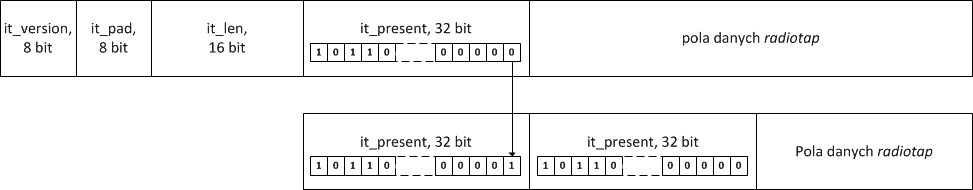
\includegraphics[width=325px]{img/RadiotapHeader}
\caption{Nagłówek \emph{radiotap}.}
\label{RadiotapHeader}
\end{center}
\end{figure}

Funkcja przetwarzająca aplikacji \emph{hop-sniffer} otrzymuje na wejściu ramkę w postaci ciągu bajtów. Ciąg ten zostaje rzutowany na strukturę odpowiadającą wyżej opisanemu składowi nagłówka i odczytywane jest pole \emph{it\_len}. Odczytywanie danych z nagłówka wymaga ekstrakcji z formatu \emph{little endian}, w którym są one kodowane. Parametr ten jest wykorzystywany do obliczenia wskaźnika na koniec nagłówka \emph{radiotap}.

Pierwszym krokiem jest odnalezienie ostatniej bitmapy \emph{it\_present} sprawdzając jej 31 bit i ewentualnie przesuwając wskaźnik o 32 kolejne. Za bitmapami znajdują się pola przechowujące dane w naturalnym porządku binarnym (co 8, 16, 32 itd. bitów). Są one rozmieszczane według tego samego porządku co odzwierciedlające je numery wewnątrz map \emph{it\_present}.

Następnie program pomiarowy przegląda dostępne bitmapy i dla każdego kolejnego, ustawionego bitu rozpakowuje odpowiadające mu pole danych. Przeglądanie bitmapy od najmniej znaczącego bitu polega na odjęciu od niej liczby 1 i wykonania operacji XOR między tablicą wynikową i wejściową. W ten sposób program otrzymuje bitmapę z ustawionym jedynie aktualnie najmniej znaczącym bitem. W celu określenia odpowiadającego mu pola \emph{radiotap} należy obliczyć na której pozycji w 32-bitowym słowie się on znajduje. Odnalezienie pozycji realizowane jest za pomocą zagnieżdżonego makra, które wykonuje przesunięcia bitowe w prawo sprawdzając czy otrzymane słowo równe jest zeru. Przesunięcia wykonywane są kolejno połowiąc pozostałe do sprawdzenia słowo, czyli kolejno o 16, 8, 4 i 2 bity. Jeśli przesunięcie wyzerowało tablicę oznacza to, że bit znajduje się na numerze pozycji mniejszym niż przesunięcie i należy ponownie wywołać makro dla tej samej tablicy przesuwając o połowę mniej bitów. Otrzymanie słowa niezerowego oznacza, że numer bitu jest wyższy niż przesunięcie. W tym przypadku można zwrócić sumę liczby przesuniętych bitów (szukany numer jest większy) i wywołania makra przesuwającego o dwukrotnie mniejszą ilość bitów, ale dla aktualnego (już przesuniętego) słowa. Jest to implementacja wzorowana na algorytmie wyszukiwania binarnego opartego na idei \emph{dziel i zwyciężaj} co sugeruje jej działanie w czasie logarytmicznym. 

Specyfikacja \emph{radiotap} zakłada, że programista znający nazwę pola zna również jego rozmiar. Pola danych rozmieszczone są zgodnie z naturalnym porządkiem binarnym. Oznacza to, że odczytując słowo określonej wielkości należy sprawdzić, czy mieści się ono w do tej pory przetworzonym fragmencie danych całkowitą liczbę razy. Jeśli tak nie jest to słowo należy odczytać z pozycji znajdującej się o brakującą liczbę bitów dalej, gdyż program trafił na wypełnienie (ang. \emph{padding}). Jest to przyjęty standard konstrukcji nagłówka \emph{radiotap}, więc \emph{hop-sniffer} również go respektuje. Przykładowo (\ref{RadiotapUnpack}), jeśli do tej pory program odczytał trzy pola o rozmiarze 8 bitów i otrzymuje polecenie odczytania słowa 16-bitowego to powinno być ono odczytane z adresu (uznając początek przestrzeni danych za 0) 32, a nie 24. 

Do rozpakowywania pól danych nagłówka \emph{radiotap} służy struktura \emph{unpacker} (\ref{code:Unpacker}). Pole \emph{u\_buf} inicjowane jest przez adresem pierwszego bajtu za ostatnią bitmapą \emph{it\_present}, \emph{u\_next} za pomocą  wskaźnika na bajt za ostatnim odczytanym słowem, a \emph{u\_len} jest różnicą wskaźnika na początek ramki i ostatnią bitmapę. 

\lstset{caption={Struktura \emph{unpacker}.}, label={code:Unpacker}}
\begin{lstlisting}[frame=tb]
struct unpacker {
        /** Pointer to the beginning of radiotap data fields area of packet. */
	u_int8_t					*u_buf;
        /** Pointer to the next packet area that was not yet extracted */
	u_int8_t					*u_next;
        /** Length of the radiotap data fields area */
	size_t						 u_len;
};
\end{lstlisting}

Po odczytaniu każdego słowa zgodnie z wyżej opisanymi regułami wskaźnik \emph{u\_next} przenoszony jest do przodu o jego długość. Wskaźnik na początek fragmentu danych służy do obliczania ewentualnych wypełnień (ang. \emph{padding}), a długość fragmentu do kontroli poprawności (jako warunek zatrzymujący przetwarzanie).

Odczytanie z bitmapy ustawionego bitu na pozycji 1 oznacza atrybut \emph{IEEE80211\_RADIOTAP\_FLAGS}, który zgodnie ze specyfikacją ma 8 bitów. Po rozpakowaniu jest on porównywany z maską \emph{0x10} (właściwość oznaczająca dodatkowy odstęp za nagłówkiem 802.11) i \emph{0x20} (ramka posiada fragment FCS). W pierwszym przypadku program ustawia zmienną \emph{pad} na wartość 1, w drugim zmienną \emph{fcslen} na wartość 4. Obydwie zmienne przekazywane są do procedury przetwarzania ramki standardu 802.11, gdzie będą potrzebne. 

Nagłówek \emph{radiotap} przechowuje również szczegółowe informacje dotyczące częstotliwości i mocy nadawania interfejsu przez, który został utworzony. Właściwość ta nie ma zastosowania w pomiarze roamingu 802.11, ale może być przydatna w bardziej skomplikowanych scenariuszach. Przetwarzanie nagłówka udostępnia więcej \emph{meta-danych} dotyczących kanału komunikacyjnego co stanowczo przemawia na jego korzyść. 

\subsubsection{Przetwarzanie nagłówka standardu \emph{802.11}.}

Wskaźnik \emph{packet} na początek migawki przechwyconej ramki (\ref{RadiotapWifi}) trafia na wejście funkcji przetwarzania nagłówka standardu 802.11 po przesunięciu o \emph{it\_len} bitów w przód. Tym samym powinien wskazywać na początek elementu FC (ang. \emph{Frame control}). Do funkcji przekazane zostają również wartości zmiennych \emph{pad} i \emph{fcslen} wyliczone w procesie przetwarzania nagłówka \emph{radiotap}. 

\begin{figure}[htb]
\begin{center}
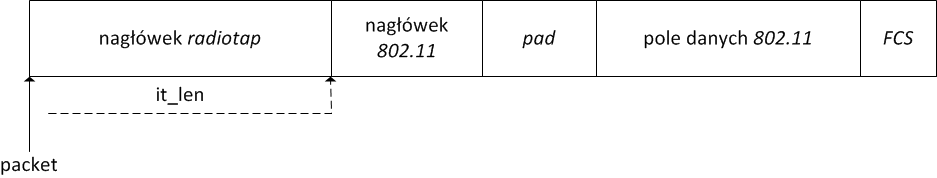
\includegraphics[width=312px]{img/RadiotapWifi}
\caption{Przesunięcie wskaźnika na początek ramki poza nagłówek \emph{radiotap}.}
\label{RadiotapWifi}
\end{center}
\end{figure}

Na podstawie danych uzyskanych z pakietu na tym etapie podejmowane są główne kroki procedury pomiarowej. Scenariusz pomiaru można rozumieć jako globalną strukturę, której pola wypełniane są w zależności od przepływu programu w wyniku wykrytego zdarzenia. Część struktur jest globalna, gdyż jest to bardziej wydajne niż przekazywanie ich bardzo głęboko w zagnieżdżonych wywołaniach funkcji, a taką właśnie strukturę ma program \emph{hop-sniffer}. 

Zgodnie z ustaleniami procedury pomiaru roamingu stacji klienckiej program powinien wykrywać dwa typy zdarzeń:
\begin{itemize}
\item[--] Odebranie ramki typu \emph{MGMT} i podtypu \emph{Association Response}.
\item[--] Odebranie ramki typu \emph{MGMT} i podtypu \emph{Disassociation}.
\end{itemize}
Sterują one przebiegiem obserwacji zjawiska, które posiada trzy zidentyfikowane stany:
\begin{enumerate}
\item Stan asocjacji z początkowym punktem dostępowym.
\item Stan przełączania kanału radiowego.
\item Stan asocjacji z docelowym punktem dostępowym.
\end{enumerate}
Stanom tym odpowiadają dobrze zdefiniowane zdarzenia. Odebranie ramki typu \emph{Association Response} z adresem źródłowym MAC początkowego punktu dostępowego wprowadza scenariusz pomiarowy w stan pierwszy. Sytuacja ta zmienia się po odebraniu ramki typu \emph{Disassociation} z adresem źródłowym MAC stacji klienckiej. Oznacza to, że stacja rozpoczęła proces roamingu i tym samym wprowadziła procedurę pomiarową w stan drugi. Ostatecznie pomiar kończy wejście scenariusza w stan trzeci spowodowane odebraniem ramki typu \emph{Association Response} z adresem źródłowym MAC docelowego punktu dostępowego, który potwierdza asocjację przybywającej stacji klienckiej.

Pierwszą czynnością jest ekstrakcja 16-bitowego pola FC (ang. \emph{Frame control}). Znajduje się ono na początku nagłówka, ale podczas rzutowania należy obsłużyć kodowanie \emph{litte endian}.

Aplikacja \emph{hop-sniffer} rozpoczyna przetwarzanie pola FC od ekstrakcji typu pakietu. W pomiarze roamingu 802.11 biorą udział jedynie ramki typu \emph{T\_MGMT}. Odczytanie typu odbywa się za pomocą makra. Wykonywane jest przesunięcie wskaźnika na pole FC poza znacznik protokołu, czyli o 2 bajty w lewo i zastosowanie do niego maski bitowej \emph{0x3}, która odczytuje 2 pierwsze bity ramki. Jeśli odczytane bity wynoszą \emph{0x0} (typ ramek MGMT) to program kontynuuje obsługę. Ramki nie będące typu \emph{T\_MGMT} są porzucane. 

Kolejnym krokiem jest rozgałęzienie przepływu programu na obsługę wybranych podtypów ramek \emph{MGMT}. Stosuję instrukcję warunkową \emph{switch} z argumentem będącym odczytanym podtypem ramki. Makro ekstrakcji podtypu dokonuje przesunięcia wskaźnika na pole FC o 4 bajty w lewo (pozbywa się znacznika protokołu i typu ramki) i stosuje maskę \emph{0xF}, która oznacza odczytanie ostatnich 4 bitów.

\begin{figure}[htb]
\begin{center}
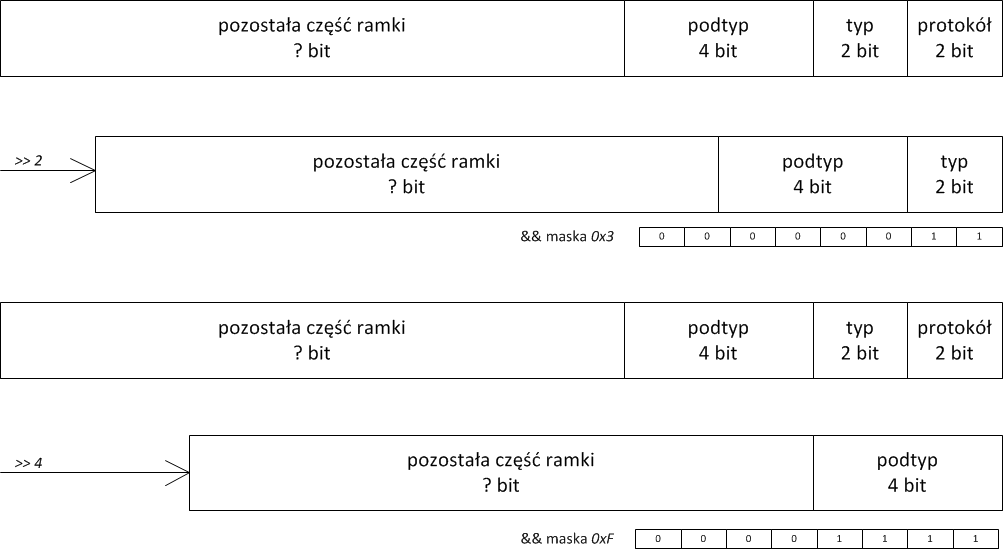
\includegraphics[width=333px]{img/TypeSubtype}
\caption{Ekstrakcja typu i podtypu z nagłówka \emph{802.11}.}
\label{TypeSubtype}
\end{center}
\end{figure}

Ostatnią brakującą daną jest adres źródłowy MAC obsługiwanego pakietu. Najłatwiej dostać się do tej informacji poprzez rzutowanie otrzymanego w argumentach wywołania funkcji wskaźnika na początek nagłówka standardu 802.11 typu \emph{MGMT} na jego reprezentację w postaci struktury danych języka \emph{C} (\ref{code:MgmtHeader}). Krok ten ułatwia dostęp do dwóch 6-bajtowych tablic \emph{sa} i \emph{da} odpowiadających źródłowemu i docelowemu adresowi MAC ramki. Pozostałe pola są zgodne ze specyfikacją i odpowiadają kolejno polu kontrolnemu, polu \emph{duration} odpowiadającemu pozostałemu czasowi z tablicy \emph{NAV}, polu \emph{BSSID} (ang. \emph{Basic Service Set Identifier}) i numerowi kontrolnemu sekwencji.

\lstset{caption={Struktura \emph{mgmt\_hdr}.}, label={code:MgmtHeader}}
\begin{lstlisting}[frame=tb]
struct mgmt_hdr
{
        u_int16_t fc;
        u_int16_t duration;
        u_int8_t da[6];
        u_int8_t sa[6];
        u_int8_t bssid[6];
        u_int16_t seq_ctrl;
};
\end{lstlisting}



\subsubsection{Przełączanie kanału radiowego stacji pomiarowej.}

Podstawową charakterystyką interfejsu karty radiowej jest jego praca wyłącznie na jednej częstotliwości w danej chwili. Popularne programy przechwytywania ramek komunikacji bezprzewodowej (np. \emph{Wireshark}) udostępniają opcję ciągłej zmiany kanału pracy w celu obrazowania ruchu w całym spektrum dostępnym w medium transmisyjnym (ang. \emph{channel hopping}). Z punktu widzenia aplikacji \emph{hop-sniffer} zachowanie takie utrudniałoby i wprowadzało zakłamania kalkulacji opóźnień wybranych zjawisk. Nie zmienia to faktu, że w obserwacji przełączania częstotliwości pracy podczas roamingu 802.11 potrzebna jest jednorazowa zmiana kanału interfejsu urządzenia przechwytującego.     

Jednym z możliwych rozwiązań, które wyklucza potrzebę przełączania kanału jest użycie dwóch kart radiowych pracujących odpowiednio na częstotliwości każdego z punktów dostępowych biorących udział w eksperymencie. Ideą programu \emph{hop-sniffer} jest jednak możliwość uruchomienia na niewielkim komputerze przenośnym i łatwa implementacja procedur pomiarowych w oparciu o pojedynczy interfejs przechwytujący. 

Zastosowane rozwiązanie jest zgodne z założeniem o przeprowadzaniu scenariusza pomiarowego w odpowiedzi na wykryte zdarzenia (ramki protokołu) i wykorzystuje metodę jawnego przełączenia kanału pracy karty radiowej. Zastosowałem udostępniany przez sterownik interfejs wywołań systemowych IOCTL za pomocą, którego program nasłuchujący wystosowuje polecenie SIOCSIWFREQ służące do wprowadzenia urządzenia w podaną w jednostkach hertz częstotliwość pracy. 

Procedurę można podzielić na następujące fazy:
\begin{enumerate}
\item Otwarcie gniazda, które umożliwi wywołanie polecenia.
\item Przygotowanie argumentów wywołania w postaci akceptowanej przez polecenie.
\item Wywołanie IOCTL SIOCSIWFREQ w odpowiedzi na przetworzenie ramki typu \emph{Disassociation}.
\end{enumerate}

Program dąży do otwarcia gniazda AF\_INET (ang. \emph{Internet socket}) dostępnego na systemach Linux. Przewidziana jest też możliwość rozwoju i przyszłej przenośności aplikacji w postaci prób stworzenia innych użytecznych gniazd (IPX, AX.25, APPLETALK) w wypadku niedostępności gniazda typu \emph{Berkeley socket}. Otwarcie następuje z parametrem SOCK\_DGRAM niezbędnym do wywołania typu IOCTL.

Argumentem wywołania jest struktura \emph{iwreq} będąca zmodyfikowaną wersją \emph{ifreq} posiadającą dodatkowe elementy unii \emph{u} w tym pole \emph{freq}. Jest to pole typu \emph{iw\_freq} rozdzielające wartość częstotliwości (daną w postaci zmiennoprzecinkowej) na mantysę i wykładnik, gdyż jądro nie udostępnia arytmetyki zmiennoprzecinkowej.

% Wzory na ekstrakcję m i e!

Jeśli podczas przetwarzania wykryta zostanie ramka typu \emph{Disassociation} to program \emph{hop-sniffer} przełącza kanał interfejsu nasłuchującego na częstotliwość nowego punktu dostępowego w celu przechwycenia stempla czasowego momentu asocjacji stacji klienckiej i tym samym zakończenia roamingu 802.11.


\begin{figure}[htb]
\begin{center}
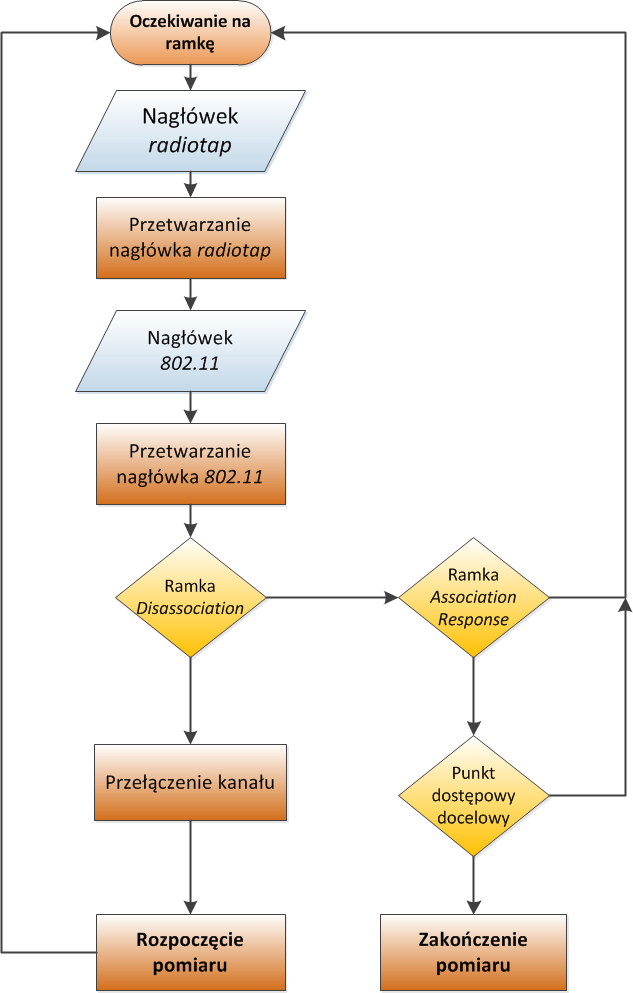
\includegraphics[width=210px]{img/FlowDiagram}
\caption{Diagram przepływu sterowania programu \emph{hop-sniffer}.}
\label{FlowDiagram}
\end{center}
\end{figure}























